\documentclass{beamer}
% Prévoir à peu près un transparent par minute d'exposé.
% Deux ou trois sections semble être une bonne chose.
\mode<presentation>
{
	\usetheme{Warsaw}
	\setbeamercovered{highly dynamic}
	\setbeamercovered{invisible}
}

\usepackage[english]{babel}
\usepackage[utf8]{inputenc}
%\usepackage{hyperref}

\setbeamersize{text margin left=20pt}
\setbeamersize{text margin right=20pt}

\defbeamertemplate*{footline}{infolines theme}
{
	\leavevmode%
	\hbox{%
		\begin{beamercolorbox}[wd=.33\paperwidth,ht=2.25ex,dp=1ex,center]{author in head/foot}%
			\usebeamerfont{author in head/foot}G. Lesauvage
		\end{beamercolorbox}%
		\begin{beamercolorbox}[wd=.33\paperwidth,ht=2.25ex,dp=1ex,center]{title in head/foot}%
			\usebeamerfont{title in head/foot}\insertshorttitle
		\end{beamercolorbox}%
		\begin{beamercolorbox}[wd=.33\paperwidth,ht=2.25ex,dp=1ex,right]{date in head/foot}%
			\usebeamerfont{date in head/foot}november 17th, 2009\hspace*{2em}
			\insertframenumber{}/\inserttotalframenumber\hspace*{2ex}
		\end{beamercolorbox}
	}%
	\vskip0pt%
}

\date{\tiny november 17th, 2009}
\title[MajecSTIC 2009]
{
	Gestion dynamique des activités des chariots cavaliers sur un terminal portuaire à conteneurs en environnement incertain\\
	- approche par intelligence collective -
}

\author
{
	G. Lesauvage
}

\institute[UFR ST Le Havre]
{
	
 \begin{columns}
 		\begin{column}[l]{6cm}
 			\begin{center}
 			
\includegraphics[height=.1\textheight]{fig/logouniversiteduhavre.png} \\
 			\tiny\textit{Unit\'{e} de Formation et de Recherche des Sciences et Techniques}
 			\end{center}
 		\end{column}
 		\begin{column}[r]{6cm}
 			\begin{center}
 			
\includegraphics[height=.1\textheight]{fig/logolitis.png} \\
 			\tiny\textit{Laboratoire d'Informatique et du Traitement de l'Information et des Syst\`{e}mes}
 			\end{center}
 		\end{column}
 	\end{columns}

 	
}

\normalsize

 \AtBeginSection[Plan]
 {
 \begin{frame}<beamer>
 \frametitle{Plan}
 \tableofcontents[currentsection]
 \end{frame}
 }
\setbeamertemplate{blocks}[rounded][shadow=true]
\subject{MajecSTIC 2009 Avignon}
\begin{document}

\begin{frame}
\titlepage
\end{frame}

\begin{frame}
\frametitle{Plan}
\tableofcontents
\end{frame}


\section{Description du système}
\subsection*{CALAS}
\begin{frame}
\frametitle{Le projet CALAS}
\begin{columns}
    \begin{column}[l]{5.5cm}	
	\begin{itemize}
		\item Système de mesure laser
		\item 2 principales entreprises : 
			\begin{itemize}
			 \item \textit{Laser Data Technology Terminal}
	 		 \item Terminaux de Normandie
			\end{itemize}
		
		 \item 2 principaux laboratoires : 
			 \begin{itemize}
			    \item LMAH
			    \item LITIS
			  \end{itemize}
	\end{itemize}
    \end{column}
    \begin{column}[r]{4.5cm}
		\begin{flushright}
		  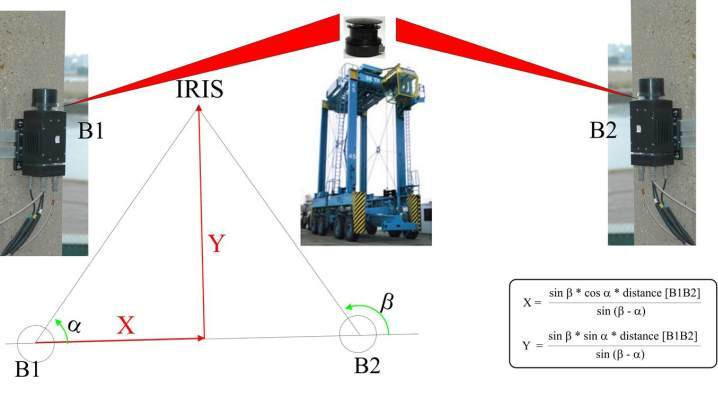
\includegraphics[height=.37\textheight]{fig/angles.jpg}
		\end{flushright}
    \end{column}
 \end{columns}	
	\begin{block}{Objectifs du projet CALAS : }
		\begin{minipage}[]{\columnwidth}
			Connaître l'état du terminal en temps réel, c'est-à-dire à la fois la position des conteneurs et celle des engins de manutention.
		\end{minipage}
	\end{block}
	

\end{frame}
\subsection*{Terminal à conteneurs}
\begin{frame}
\frametitle{Description d'un terminal}

 	\begin{columns}
 	 	\begin{column}[l]{4.5cm}
			\begin{itemize}
				\item Plateforme de transit de conteneurs
				\item 3 principales zones : 
				\begin{itemize}
 					\item Zone maritime
					\item Zone de stockage
					\item Zone terrestre
				\end{itemize}
			\end{itemize}
		\end{column}
 	 	\begin{column}[r]{7.5cm}
			\begin{flushright}
				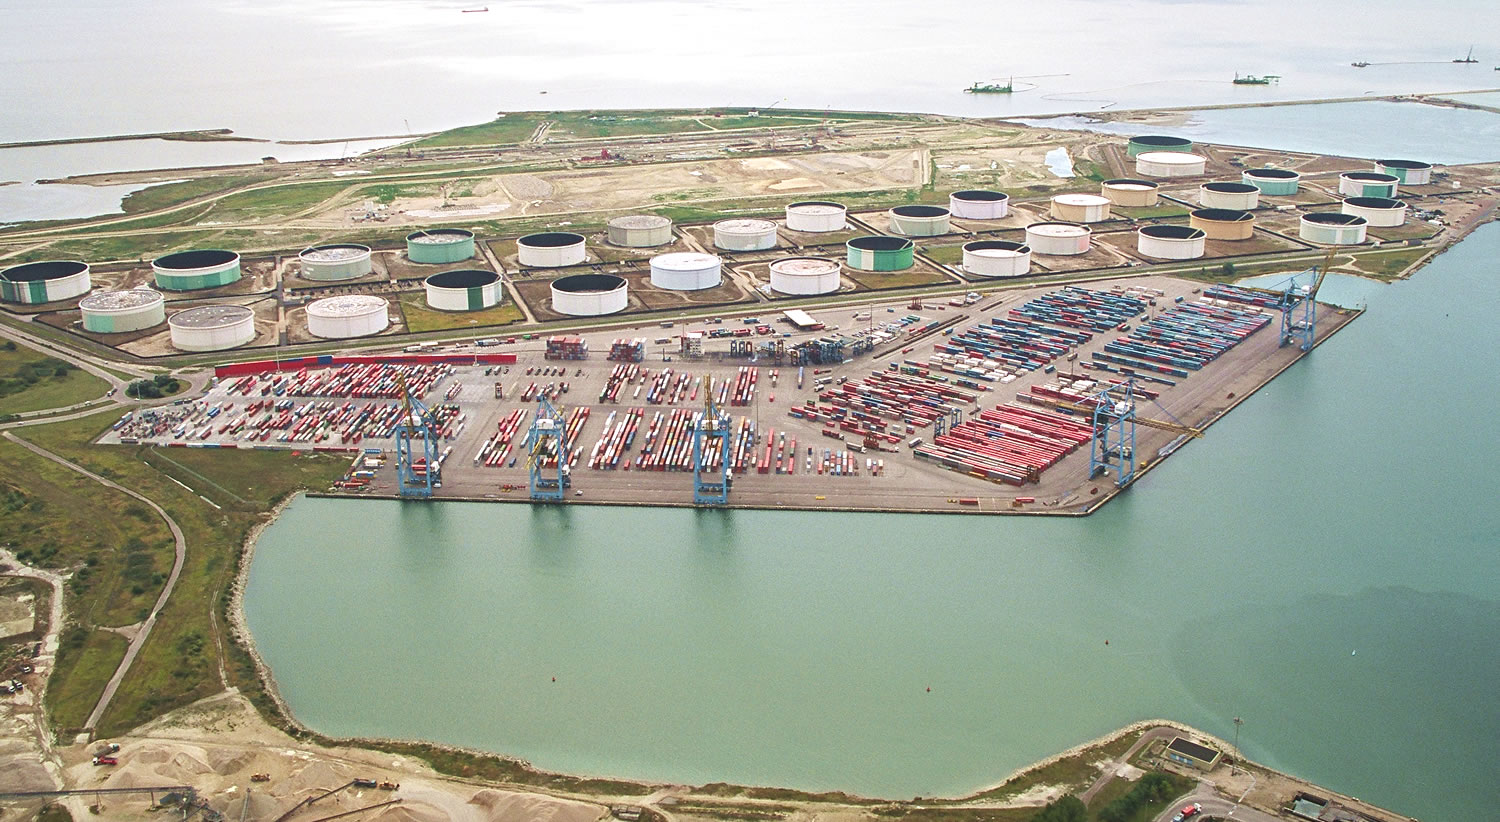
\includegraphics[height=.55\textheight]{fig/terminalDeNormandie.jpg}
			\end{flushright}
		\end{column}
 	\end{columns}
\begin{itemize}
\item La zone de sctockage est composée de longues travées de conteneurs empilés sur plusieurs niveaux
\end{itemize}
\end{frame}
\begin{frame}
 \frametitle{Engins de manutention}
\begin{columns}
  \begin{column}[l]{8cm}
    \begin{itemize}
    \item Les chariots cavaliers sont des engins de manutention qui peuvent transporter un conteneur à la fois
    \item Ils sont capable d'enjamber une travée de conteneurs et de prendre (déposer) un conteneur sur le sommet d'une pile
    \item Une mission consiste à déplacer un conteneur d'un point $A$ à un point $B$ sur le terminal
    \end{itemize}
  \end{column}
  \begin{column}[r]{3cm}
	\begin{flushright}
	    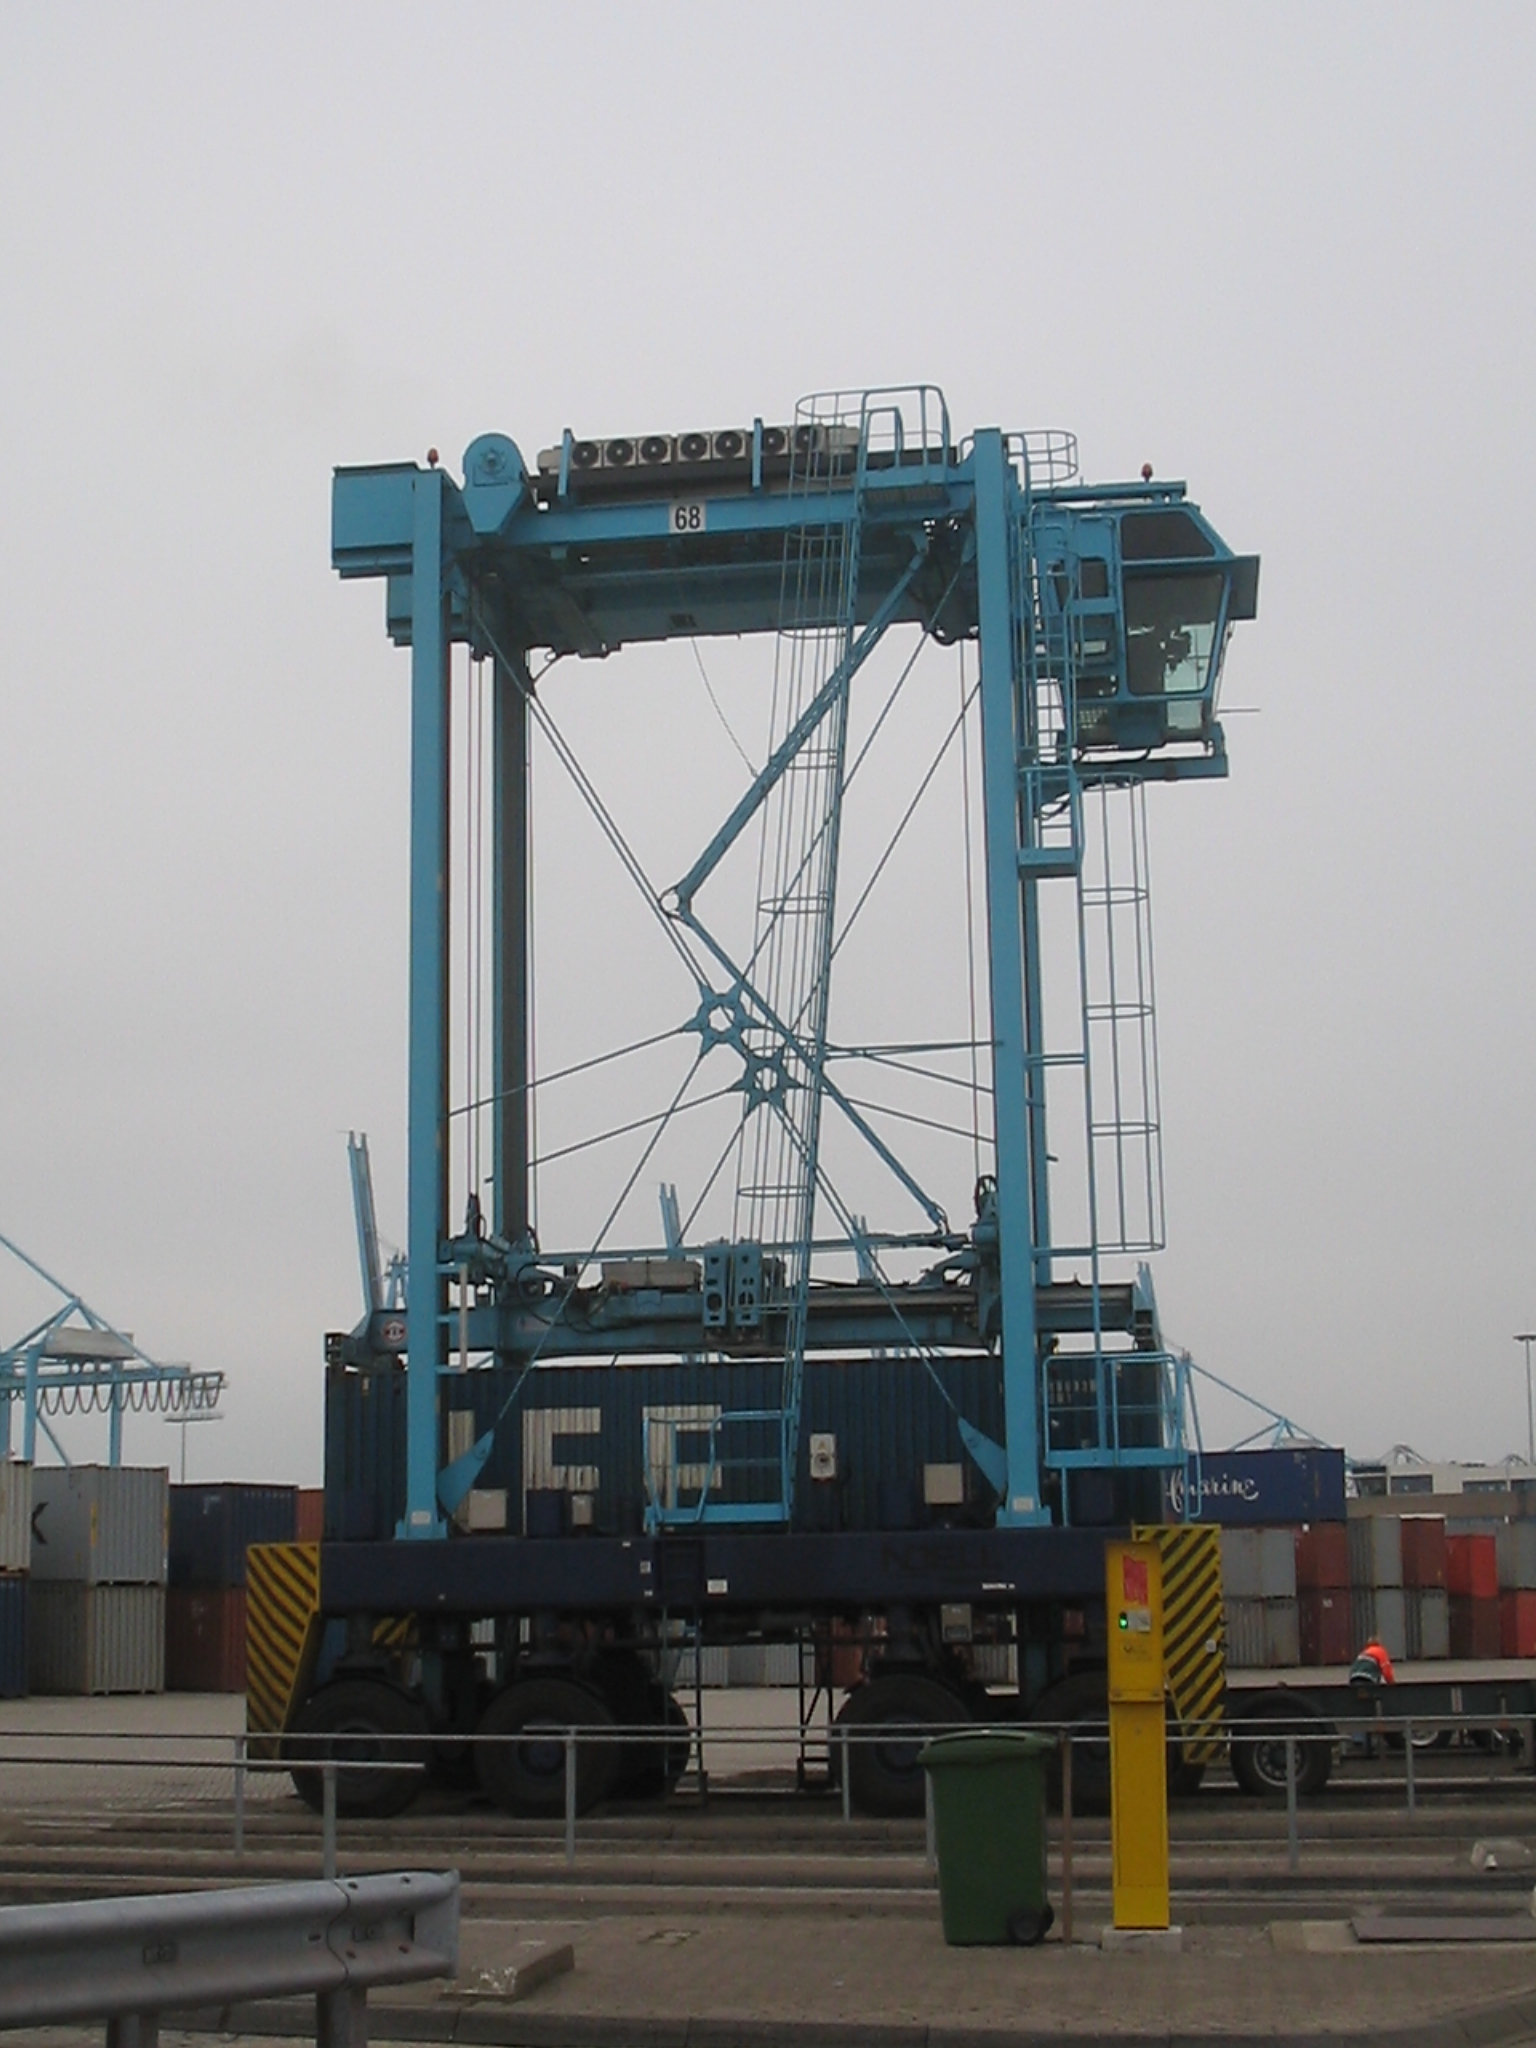
\includegraphics[height=.5\textheight]{fig/Containerlift_straddle_carrier.jpg}
	\end{flushright}
  \end{column}
\end{columns}	
\end{frame}

\begin{frame}
\frametitle{Activités des chariots cavaliers}
\begin{columns}
  \begin{column}[l]{5.5cm}
	3 types de missions : 
	 \begin{itemize}
	  \definecolor{vert}{rgb}{0.0,0.5,0.0}
	  \definecolor{bleu}{rgb}{0.0,0.0,0.5}
	  \definecolor{jaune}{rgb}{0.75,0.75,0.0}
	  \item Préparer le (dé)chargement d'un \textcolor{vert}{navire}
	  \item Préparer le (dé)chargement d'un \textcolor{bleu}{camion} ou d'un \textcolor{bleu}{train}
	  \item Optimiser la zone de \textcolor{jaune}{stockage}
	\end{itemize}
\end{column}
  \begin{column}[r]{5.5cm}
	\begin{flushright}
	    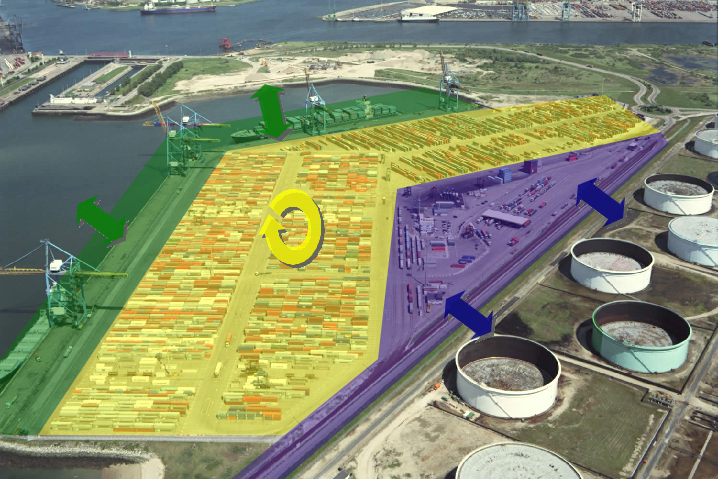
\includegraphics[height=.5\textheight]{fig/threeKindsOfMissions.png}
	\end{flushright}
  \end{column}
\end{columns}
\end{frame}

\subsection*{Dynamicité du système}
\begin{frame}
\frametitle{Système ouvert}
	\begin{columns}
		\begin{column}[l]{8cm}
			Un système ouvert implique un environnement incertain.

			Les flots entrants et sortants : 
			\begin{itemize}
				\item ne dépendent pas uniquement du système lui-même
				\item affectent le système et le conduisent dans un nouvel état
			\end{itemize}
		\end{column}
		\begin{column}[r]{4cm}
			\begin{center}
				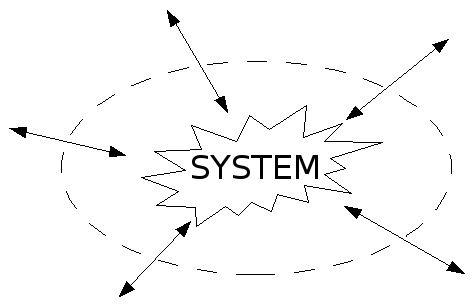
\includegraphics[height=.30\textheight]{fig/openSystem.png}
			\end{center}
	 	\end{column}
	\end{columns}
\end{frame}
\begin{frame}
\frametitle{Environnement incertain}
	Il existe plusieurs événements imprévisibles tels que :
	  \begin{itemize}
	  \item L'arrivée des missions
	  \item L'heure d'arrivée des camions, des  trains, et des navires
	  \item Les déconnections au sein du réseau routier (et ferroviaire)
	  \item Les pannes des engins de manutention
	  \item Le comportement humain %bien insister là-dessus et dire que seuls les conducteurs ont le pouvoir de respecter le plan d'ordonnancement
	\end{itemize}
\end{frame}


\section{Problèmes de tournées de véhicules : état de l'art}

\subsection*{Problème de tournées de véhicules avec fenêtre de temps}

\begin{frame}
\frametitle{VRPTW\cite{Berbeglia07}}
	\begin{columns}
	 	\begin{column}[l]{6cm} \begin{center}
			\begin{itemize}
 				\item \small{\textbf{V}ehicle \textbf{R}outing \textbf{P}roblem}
			\end{itemize} \end{center}
	 	\end{column}
	 	\begin{column}[r]{6cm} \begin{center}
			\begin{itemize} 
				\item \small{\textbf{T}ime \textbf{W}indows}
			\end{itemize} \end{center}
	 	\end{column}
	\end{columns}
	\begin{block}{Objectif}
		\begin{center} Optimiser les routes de livraisons de chaque véhicule\end{center}
	\end{block}
		
	\begin{exampleblock}{exemple de VRPTW : la fabrique de jouets}
		\small{\begin{itemize}
			\item Une usine fabrique des jouets et des véhicules doivent les livrer à un ensemble de points de vente
			\item Les boutiques sont réparties sur tout le territoire et les marchandises sont transportées par camion
			\item Chaque camion a une capacité limitée et débute sa tournée au dépot
			\item les livraisons doivent intervenir au cours d'un intervale défini et si un camion arrive trop tot, il devra attendre
		\end{itemize}}
	\end{exampleblock}
\end{frame}


\subsection*{Problème dynamique de tournées de véhicules}
\begin{frame}
	\frametitle{DVRPTW\cite{Mitrovic01}}
	\begin{itemize}
 		\item Version dynamique du VRP
	\end{itemize}
	\begin{block}{Objectif}
		\begin{center}
			Optimiser les nouvelles routes de chaque véhicule sans tout recalculer de zéro
		\end{center}
	\end{block}	
	
	\begin{exampleblock}{La fabrique dynamique de jouets}
		\begin{itemize}
			\item problème statique de la fabrique de jouets
			\item même si une tournée est déjà en cours les boutiques peuvent demander de nouvelles livraisons
		\end{itemize}
	\end{exampleblock}
\end{frame}

\subsection*{Problème (dynamique) de collecte et de livraison}
\begin{frame}
 \frametitle{(D)PDP}
	\begin{itemize}
	 \item DVRP où les marchandises doivent d'abord être collectées avant d'être livrées
	\end{itemize}
	
	\begin{block}{Objectif}
		\begin{center}
			Optimiser à la fois les routes de collecte et de livraison
		\end{center}
	\end{block}	
	\begin{exampleblock}{Problème du postier}
		\begin{itemize}
			\item Une entreprise postale emploie un ensemble de postiers
			\item Ils doivent collecter le courrier dans les boîtes de la compagnie
			\item Puis, ils doivent livrer les clients aussi vite que possible
		\end{itemize}
	\end{exampleblock}

\end{frame}

\subsection*{Problème dynamique de collecte et livraison des chariots cavaliers avec fenêtre de temps}
\begin{frame}
\frametitle{DSCPDPTW}
	\begin{itemize}
 		\item Pickup and Delivery Problem
		\item Capacité unitaire
		\item Fenêtre de temps : \small dépend à la fois des chariots cavaliers et des camions/trains/navires\normalsize
		\item Dynamique : 
			   \begin{itemize}
			    \item Un plan peut changer à chaque instant : \small les vehicules commencent leur tournée de n'importe où (pas forcément du dépot)\normalsize
			    \item Pannes des chariots cavaliers : \small le nombre de ressources peut changer\normalsize
			    \item Heure d'arrivée des camions/trains/navires : \small il est impossible d'être sûr qu'ils vont respecter leur fenêtre de temps\normalsize
			    \item ...
			    \begin{center}  Une solution calculée doit pouvoir être annulée à chaque instant ! \end{center}
			    \end{itemize}
	\end{itemize}
\end{frame}
\begin{frame}{DSCPPDTW (2)}
	\begin{itemize}
	 \item 2 problèmes : 
		\begin{itemize}
 			\item Minimiser les déplacements des chariots cavaliers : problème de plus court chemin
			\item Minimiser le temps d'attente des clients : problème d'ordonnancement
		\end{itemize}
	\end{itemize}
	
	
	\begin{alertblock}{Dépendances des problèmes}
		\begin{tabular}{*{3}{l}}
			ordonnancement approprié & $\Rightarrow$ & concept du plus court chemin\\
			plannifier des plus court chemins & $\Rightarrow$ & optimiser l'ordonnancement
		\end{tabular}
	\end{alertblock}	
\end{frame}


\section{Ant Colony et gestion des chariots cavaliers}
\subsection*{Ant Colony : description générale}
\begin{frame}
\frametitle{Ant Colony Optimization\cite{Dorigo91}}
	\begin{itemize}
 		\item ACO est une méta-heuristique
		\item ACO fait émerger une solution grâce aux parcours locaux d'insectes artificiels dans l'espace de recherche
		\item ACO est adapté à la nature dynamique du problème :
		\begin{itemize}
		     \item Rétro-action positive : les fourmis déposent de la phéromone en fonction de la qualité de la solution
		     \item Rétro-action négative : les pistes de phéromone s'évaporent progressivement
		\end{itemize}
	\end{itemize}
	
\end{frame}
\subsection*{Ant Colony et ordonnancement}
\begin{frame}
\frametitle{Ordonnancement grâce à Ant Colony}
 	\small
	Ant Colony avec \textbf{une colonie} fourni une liste ordonnée de missions à accomplir
	\pause
	\begin{block}{Problème}
		\begin{center}
			Comment affecter une mission à un chariot cavalier en particulier ?
		\end{center}
	\end{block}

	
	\pause
	
	\begin{block}{Fourmis colorées\cite{Bertelle02} : }
	\begin{itemize}
 		\item chaque chariot cavalier représente une colonie avec sa propre couleur
		\item les fourmis sont attirées par la phéromone de leur propre colonie
		\item les fourmis sont repoussées par la phéromone des colonies étrangères
	\end{itemize}
	\end{block}
	 
  
	\pause
	Ant Colony avec \textbf{plusieurs colonies} fournit une liste ordonnée de missions par chariot cavalier
	\normalsize
\end{frame}
\subsection*{Modèlisation de l'ordonnancement : graphe de missions}
\begin{frame}
\frametitle{Graphe de missions}
	Le graphe orienté peut être modélisé de la façon suivante :
		\begin{itemize}
	 		\item Sommets : 
				\begin{itemize}
 					\item 1 mission = 1 sommet
					\item 1 chariot cavalier = 1 noeud coloré connecté à toutes les missions compatibles
				\end{itemize}
 
			\item Arcs colorés :
				\begin{itemize}
					\item Compatibilité entre 2 missions pour un chariot cavalier
				\end{itemize}
		\end{itemize}

	%\begin{block}{Ordering missions}
	%	We say that mission $m_a$ is \textbf{prior} to mission $m_b$ if the time window of $m_a$ starts before the one of $m_b$
	%\end{block}

	\begin{block}{Compatibilité des missions}
		Une mission $m_a$ est dite \textbf{compatible} avec une mission $m_b$ si la fenêtre de temps de $m_a$ commence avant celle de $m_b$
	\end{block}

\end{frame}
\begin{frame}
 \frametitle{Exemple de construction d'un graphe de missions (1)}
	\begin{exampleblock}{Exemple}
		\begin{itemize}
		 \item Missions : \\
		\begin{center}
			\begin{tabular}{*{3}{|c|c|c}}
	 	 		\hline
		 		Nom	&	Début	&	Fin\\
				\hline
				m0	&	5:00	&	6:00 \\
				m1	&	5:30	&	6:00 \\
				m2	&	7:00	&	9:00 \\
				m3	&	6:00	&	7:30 \\
				\hline
	 		\end{tabular}
		\end{center}
		\item Chariots cavaliers : \\
		\begin{center}
			\begin{tabular}{*{3}{|c|c|c}}
	 	 		\hline
		 		Nom	&	Couleur	& Compatiblilité\\
				\hline
				s0	&	\textcolor{green}{vert}	& m0, m1, m2, m3\\
				s1	&	\textcolor{blue}{bleu}	& m0,m3\\	
				\hline
	 		\end{tabular}
		\end{center}
		
		\end{itemize}

	\end{exampleblock}
	

	
\end{frame}
\begin{frame}
	\frametitle{Exemple de construction d'un graphe de missions (2)}
	\begin{center}
		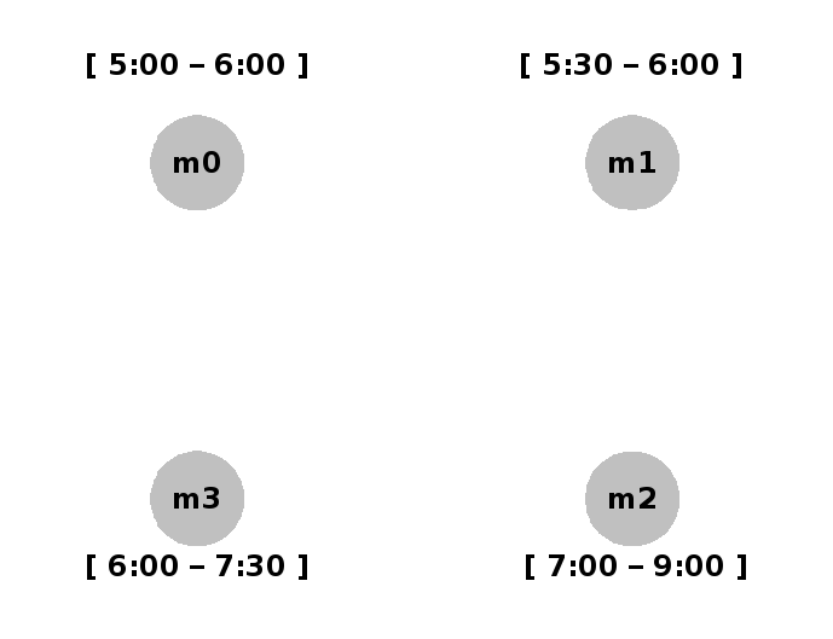
\includegraphics[height=.50\textheight]{fig/only_vertices.png} \\
	
		1 mission $\Longleftrightarrow$ 1 sommet
	\end{center}
	
\end{frame}
\begin{frame}
	\frametitle{Exemple de construction d'un graphe de missions (3)}
 	\begin{center}
 		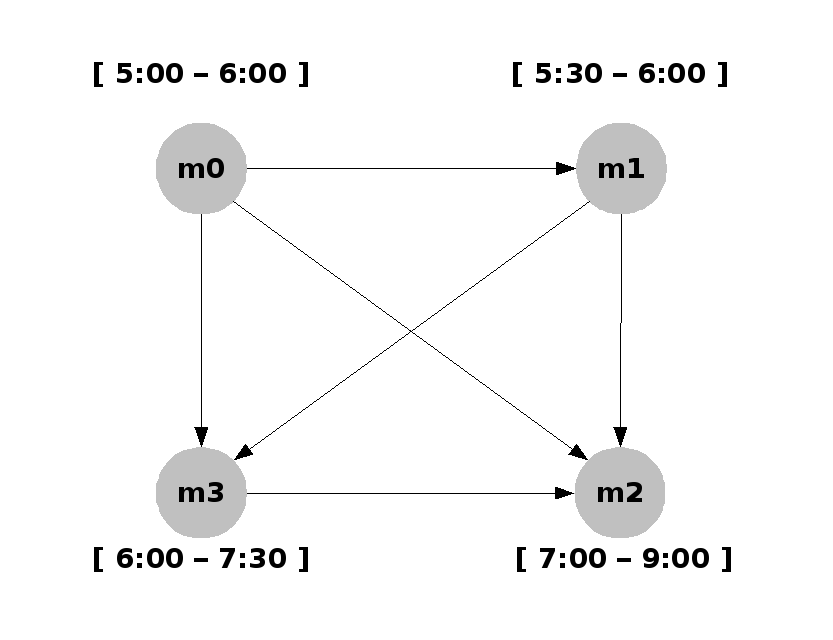
\includegraphics[height=.50\textheight]{fig/precedence.png} \\

		1 arc entre 2 missions compatibles
	\end{center}
\end{frame}
\begin{frame}
	\frametitle{Exemple de construction d'un graphe de missions (4)}
 	\begin{center}
 		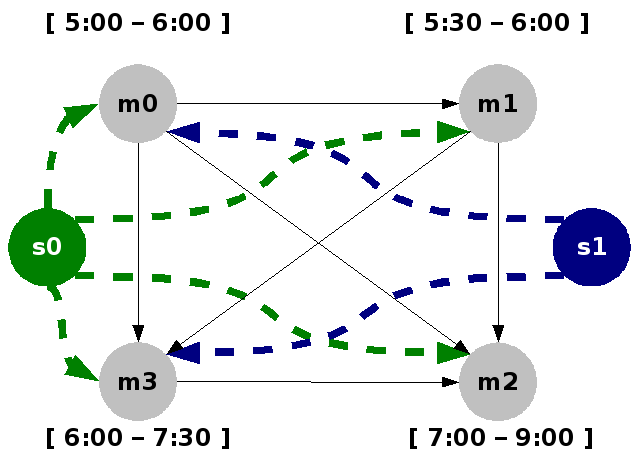
\includegraphics[height=.50\textheight]{fig/precedence_with_vehicles.png}\\
		Ajout de sommets représentant les chariots cavaliers et connection avec les missions compatibles
	\end{center}
\end{frame}
\begin{frame}
	\frametitle{Exemple de construction d'un graphe de missions (5)}
 	\begin{center}
 		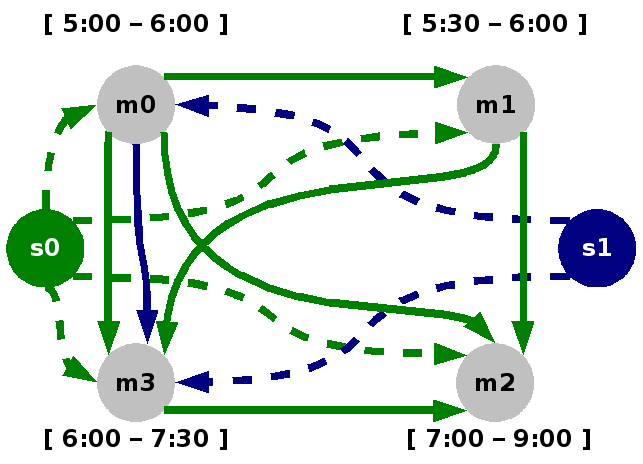
\includegraphics[height=.50\textheight]{fig/missionGraphComplet.png}\\
		Ajout ou coloration d'arcs entre les noeuds selon leur connectivité avec les véhicules
	\end{center}
\end{frame}
\subsection*{Algorithme principal}

\begin{frame}
\frametitle{Description de l'algorithme}
	\setbeamertemplate{blocks}[rounded][shadow=true]
	\small
	\begin{block}{Algorithme principal}
	\underline{début}\\
	$\vert \;$\underline{pour} chaque colonie $c$ \underline{faire}\\
	$\vert \;\vert \;$\underline{pour} chaque fourmi $a$ de $c$ \underline{faire}\\
	$\vert \;\vert \;\vert \;$choisir une destination non visitee en fonction de la trace de pheromone\\
	$\vert \;\vert \;\vert \;$se déplacer vers elle en fonction de la vitesse de $a$\\
	$\vert \;\vert \;\vert \;$déposer de la phéromone en fonction de la qualité de la destination\\
	$\vert \;\vert \;$\underline{fin pour}\\
	$\vert \;$\underline{fin pour}\\
	$\vert \;$évaporation\\
	\underline{fin}\\
	\end{block}
	\normalsize
\end{frame}
\subsection*{Solution}
\begin{frame}
\frametitle{Solution}

	\begin{itemize}
	  \item La solution correspond à la coloration des noeuds.
	  \item Lorsqu'un chariot cavalier est disponible, il choisit la mission de sa couleur qui a le taux de pheromone le plus élevé.
	  \item Les missions choisies sont supprimées du graphe et l'algolrithme continue de fonctionner.
	  \item Les noeuds des nouvelles missions sont dynamiquement ajoutés sur le graphe afin d'être pris en compte par l'algorithme.
	\end{itemize}
	
	\begin{center}
		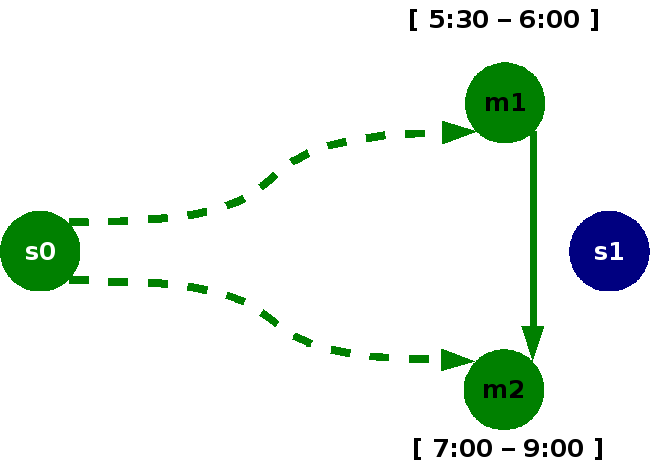
\includegraphics[height=.40\textheight]{fig/missionGraphWith2NodesRemoved.png}
	\end{center}
\end{frame}

\section{Simulateur}
\subsection*{2 vues parallèles du système}
\begin{frame}
\frametitle{2 vues parallèles du système}
	\setbeamertemplate{blocks}[rounded][shadow=true]
 	\begin{columns}
	 	\begin{column}[l]{6cm}
	 		\begin{itemize}
				 \item Implémentation du terminal
			\end{itemize}
		\end{column}
		\begin{column}[r]{6cm}
			\begin{itemize}
				  \item Modelisation d'ACO\cite{Dutot2007}
			\end{itemize}
		\end{column}
 	\end{columns}
	\begin{center} 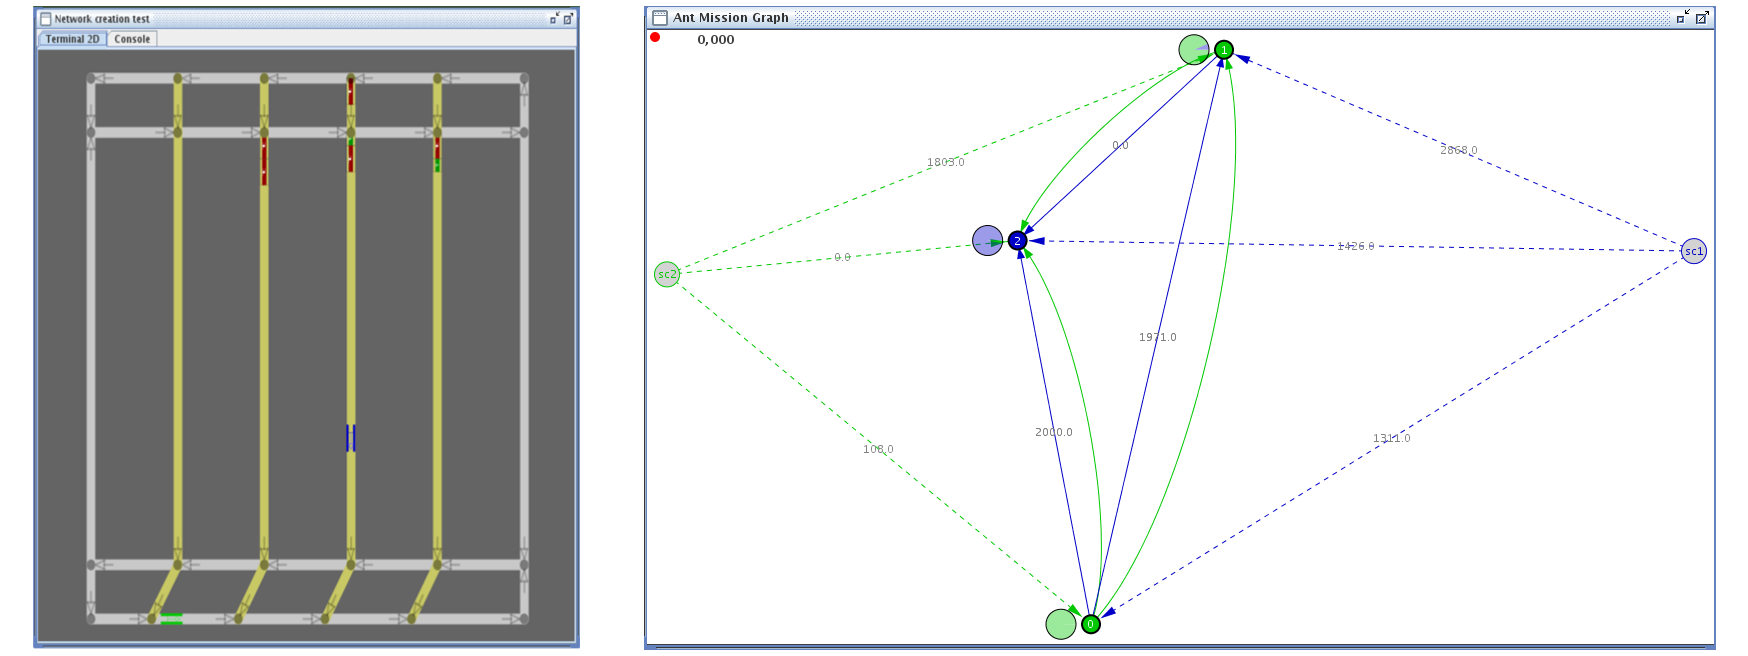
\includegraphics[height=3.7cm]{fig/terminalEtGraphe.png} \end{center}

	\begin{block}{ACO $\Longleftrightarrow$ Terminal}
		\begin{center}
			Les effets d'ACO doivent être visibles sur le terminal et l'état du terminal doit affecter le graphe de missions d'ACO
	 	\end{center}
	\end{block}
\end{frame}

\subsection*{Gestion de la dynamique}
\begin{frame}

 \frametitle{Gestion de la dynamique}
Un fichier scénario est lu tout au long de l'exécution de la simulation. Il contient des évenements dynamiques.

\begin{block}{Mesure de la dynamicité}
Selon A. Larsen\cite{Larsen00}, il est possible de quantifier la dynamicité d'un scénario grâce à ces deux formules : 
  \begin{itemize}
  \item Degree of Dynamism (dod) = $\frac{\eta_d}{\eta_s+\eta_d}$
  \item Effective Degree of Dynamism (edod) = $\; \frac{\sum_{i=1}^{\eta_d}\frac{t_i}{T}}{\eta_s+\eta_d}$
\end{itemize}

$\eta_s$ : nombre de requêtes statiques ; \\
$\eta_d$ : nombre de requêtes dynamiques.

\end{block}
\end{frame}


\section{Résultats préliminaires}
\begin{frame}
\frametitle{Résultats préliminaires}
\begin{itemize}
 \item Tester la pertinence de notre modèlisation et de notre algorithme sur des données simulées
 \item En faisant varier la dynamicité
\end{itemize}

\small
\begin{center}
	\begin{tabular}{*{5}{|l|c|c|c}}
		\hline
						& Statique& Semi-dynamique & Dynamique \\
		\hline
		$dod$				& 0 	&0.5 	& 1 	 \\
		$edod$				& 0 	&0.25	& 1 	\\
		\hline
		Fin de simulation		&22693	& 22276	& 22693   \\
		\hline		
		Fenêtres de temps dépassées	&3	&5 	& 7 \\
		\hline		
		Pénalité de dépassement		&6467	&8477	& 12485\\
		\hline
	
	\end{tabular}
\end{center}
\normalsize

%Comment
Le dépassement des fenêtres de temps ains que le temps de pénalité évoluent de la même façon que $dod$ et $edod$.

\end{frame}

\section{Conclusion}
\begin{frame}
 \frametitle{Conclusion}
	\begin{itemize}
	 \item Un problème hautement dynamique
	 \item Dynamic Pickup and Delivery Problem with Time Windows
	 \item Intelligence collective :
	 \begin{itemize}
		\item Modélisation sous forme de graphe
		\item Ant Colony System
		\item Fourmis colorées
	\end{itemize}
	 \item Un simulateur est en cours de développement et permettra de mesurer la performance de notre solution
	 \item Les résultats préliminaires confirment que notre modèle est capable de gérer la dynamicité
	\end{itemize}

	\pause
	\begin{center}
		\textbf{Merci de votre attention}
	\end{center}
\end{frame}
\tiny
\bibliographystyle{plain}
\bibliography{biblioMajecSTIC2009}
% \begin{frame}
%  \frametitle{UML modeling}
% 	\begin{figure}[center,h]
% 		\includegraphics[height=0.8\textheight]{Shemas/simplified_uml.png}
% 	\end{figure}
% \end{frame}
% 
% 
% \begin{frame}
%  \frametitle{UML modeling}
% 		\begin{figure}[center,h]
% 			\includegraphics[height=0.8\textheight]{Shemas/uml_aco.png}
% 		\end{figure}
% \end{frame}
\end{document}